\documentclass[english, doc]{apa7}\usepackage[]{graphicx}\usepackage[]{color}
% maxwidth is the original width if it is less than linewidth
% otherwise use linewidth (to make sure the graphics do not exceed the margin)
\makeatletter
\def\maxwidth{ %
  \ifdim\Gin@nat@width>\linewidth
    \linewidth
  \else
    \Gin@nat@width
  \fi
}
\makeatother

\definecolor{fgcolor}{rgb}{0.345, 0.345, 0.345}
\newcommand{\hlnum}[1]{\textcolor[rgb]{0.686,0.059,0.569}{#1}}%
\newcommand{\hlstr}[1]{\textcolor[rgb]{0.192,0.494,0.8}{#1}}%
\newcommand{\hlcom}[1]{\textcolor[rgb]{0.678,0.584,0.686}{\textit{#1}}}%
\newcommand{\hlopt}[1]{\textcolor[rgb]{0,0,0}{#1}}%
\newcommand{\hlstd}[1]{\textcolor[rgb]{0.345,0.345,0.345}{#1}}%
\newcommand{\hlkwa}[1]{\textcolor[rgb]{0.161,0.373,0.58}{\textbf{#1}}}%
\newcommand{\hlkwb}[1]{\textcolor[rgb]{0.69,0.353,0.396}{#1}}%
\newcommand{\hlkwc}[1]{\textcolor[rgb]{0.333,0.667,0.333}{#1}}%
\newcommand{\hlkwd}[1]{\textcolor[rgb]{0.737,0.353,0.396}{\textbf{#1}}}%
\let\hlipl\hlkwb

\usepackage{framed}
\makeatletter
\newenvironment{kframe}{%
 \def\at@end@of@kframe{}%
 \ifinner\ifhmode%
  \def\at@end@of@kframe{\end{minipage}}%
  \begin{minipage}{\columnwidth}%
 \fi\fi%
 \def\FrameCommand##1{\hskip\@totalleftmargin \hskip-\fboxsep
 \colorbox{shadecolor}{##1}\hskip-\fboxsep
     % There is no \\@totalrightmargin, so:
     \hskip-\linewidth \hskip-\@totalleftmargin \hskip\columnwidth}%
 \MakeFramed {\advance\hsize-\width
   \@totalleftmargin\z@ \linewidth\hsize
   \@setminipage}}%
 {\par\unskip\endMakeFramed%
 \at@end@of@kframe}
\makeatother

\definecolor{shadecolor}{rgb}{.97, .97, .97}
\definecolor{messagecolor}{rgb}{0, 0, 0}
\definecolor{warningcolor}{rgb}{1, 0, 1}
\definecolor{errorcolor}{rgb}{1, 0, 0}
\newenvironment{knitrout}{}{} % an empty environment to be redefined in TeX

\usepackage{alltt}

\usepackage[]{graphicx}
\usepackage[]{color}


\usepackage{alltt}
\usepackage{lmodern}
\usepackage{amsmath}
\usepackage{ifxetex,ifluatex}
\hypersetup{
  pdftitle={Absence of Evidence for Underspecification in Prenominal Relative Clause Attachment},
  pdflang={en-EN},
  pdfkeywords={keywords},
  hidelinks,
  pdfcreator={LaTeX via pandoc}}
  
  
\urlstyle{same} % disable monospaced font for URLs
\usepackage{graphicx}


\usepackage[utf8x]{inputenc}
\usepackage[T1]{fontenc}
\usepackage[natbibapa]{apacite}

\usepackage{xcolor}
\usepackage{hhline}
\usepackage{mathtools}
\usepackage{gb4e}\noautomath

\usepackage[normalem]{ulem}
\usepackage{makecell}

% Table formatting
\usepackage{longtable}
\usepackage{lscape}
% \usepackage[counterclockwise]{rotating}   % Landscape page setup for large tables
\usepackage{multirow}		% Table styling
\usepackage{tabularx}		% Control Column width
\usepackage[flushleft]{threeparttable}	% Allows for three part tables with a specified notes section
\usepackage{threeparttablex}            % Lets threeparttable work with longtable
\usepackage{multicol}
\usepackage{color, soul}
\usepackage{background}
\usepackage{lipsum}% just to generate filler text

\SetBgContents{Version dated \today}
%\SetBgContents{}
\SetBgScale{1}
\SetBgAngle{0}
\SetBgColor{black!40}            % color
\SetBgPosition{current page.north east}
\SetBgHshift{-3.5cm}
\SetBgVshift{-1cm}

%\def \red  {\color{red}}
%\def \redx#1 { \textcolor{red}{#1} }

\def \red  { }
\def \redx#1 { #1 }


\title{Absence of Evidence for Underspecification in Prenominal Relative Clause Attachment} %\newline\newline{\small{Version dated \today
\shorttitle{Underspecification in Prenominal RC Attachment}
\date{\today}

\author{Pavel Logačev\textsuperscript{1}, Özgur Aydın\textsuperscript{2}, Aylin Müge Tuncer\textsuperscript{3}}
\affiliation{
\vspace{0.5cm}
\textsuperscript{1} {Boğaziçi University, Istanbul, Turkey} \\
\textsuperscript{2} {Ankara University, Ankara, Turkey} \\
\textsuperscript{3} {Muğla Sıtkı Koçman University, Muğla, Turkey} }
\authornote{
%Add complete departmental affiliations for each author here. Each new line herein must be indented, like this line.
%Enter author note here.


Correspondence concerning this article should be addressed to Pavel Logačev, %, Postal address. 
E-mail: pavel.logacev@boun.edu.tr

We would like to thank three anonymous reviewers for their helpful comments and suggestions, as well as Shravan Vasishth for extensive comments on earlier versions of this work.
}
\keywords{relative clause attachment, underspecification, Turkish, sentence processing\newline\indent Word count: 6,955}
\usepackage{csquotes}
\ifxetex
  % Load polyglossia as late as possible: uses bidi with RTL langages (e.g. Hebrew, Arabic)
  \usepackage{polyglossia}
  \setmainlanguage[]{english}
\else
  \usepackage[shorthands=off,main=english]{babel}
\fi
\ifluatex
  \usepackage{selnolig}  % disable illegal ligatures
\fi
\newlength{\cslhangindent}
\setlength{\cslhangindent}{1.5em}
\newlength{\csllabelwidth}
\setlength{\csllabelwidth}{3em}
\newenvironment{CSLReferences}[2] % #1 hanging-ident, #2 entry spacing
 {% don't indent paragraphs
  \setlength{\parindent}{0pt}
  % turn on hanging indent if param 1 is 1
  \ifodd #1 \everypar{\setlength{\hangindent}{\cslhangindent}}\ignorespaces\fi
  % set entry spacing
  \ifnum #2 > 0
  \setlength{\parskip}{#2\baselineskip}
  \fi
 }%
 {}
\usepackage{calc}
\newcommand{\CSLBlock}[1]{#1\hfill\break}
\newcommand{\CSLLeftMargin}[1]{\parbox[t]{\csllabelwidth}{#1}}
\newcommand{\CSLRightInline}[1]{\parbox[t]{\linewidth - \csllabelwidth}{#1}\break}
\newcommand{\CSLIndent}[1]{\hspace{\cslhangindent}#1}






%\title{Incrementality in Pre-nominal Relative Clause Attachment}


\abstract{
Traxler et al. (1998) have found that relative clauses with ambiguous attachment are sometimes read faster than their unambiguous counterparts. Two broad classes of theories account for this phenomenon: Race-based models posit that ambiguous sentences are read faster due to a ‘race’ between several permissible analyses of the sentence. In contrast, the strategic underspecification account maintains that, under the right conditions, readers underspecify ambiguities in order to save time. We argue that the two accounts make qualitatively different predictions for structures with pre-nominal relative clauses, such as in Turkish. While the underspecification account predicts an ambiguity advantage in Turkish, race-based accounts predict the absence of such an effect. 
We present data from two reading experiments in Turkish ($N=39$ and $N=184$) in which we find no evidence for a substantial ambiguity advantage in the processing of ambiguous sentences with prenominal relative clauses and argue that this finding poses a major challenge for the strategic underspecification account.

% long version
%Traxler et al.~(1998) have found that relative clauses with ambiguous attachment are read faster than their unambiguous counterparts under certain conditions. Presently, there are two broad classes of accounts of this phenomenon: \emph{Race-based models} (van Gompel et al., 2000; Loga\v cev \& Vasishth, 2016) posit that ambiguous sentences are read faster due to a `race' between several permissible analyses of the sentence. In contrast, the \emph{strategic underspecification account} by Swets et al.~(2008) maintains that, under the right conditions, readers are capable of underspecifying ambiguities in order to save time. We argue that while the two accounts make similar predictions for languages with postnominal relative clauses, such as English, they make qualitatively different predictions for structures with prenominal relative clauses, such as in Turkish. While the underspecification account predicts an ambiguity in Turkish, race-based accounts predict the absence of such an effect.
%We present data from two reading experiments in Turkish in which we fail to find evidence for the hypothesis that sentences with ambiguous attachment are processed faster than their unambiguous counterparts. We conclude that there is no evidence for an ambiguity advantage in the processing of ambiguous sentences with prenominal relative clauses and argue that this finding poses a major challenge for the strategic underspecification account.
}
\IfFileExists{upquote.sty}{\usepackage{upquote}}{}
\IfFileExists{upquote.sty}{\usepackage{upquote}}{}
\begin{document}
\maketitle

One important question in human sentence comprehension has always been how the human parser deals with ambiguity. A central phenomenon in that regard is the ambiguity advantage, first reported by \cite{TraxlerEtAl:1998}, who found that sentences with globally ambiguous relative clause attachment such as (\ref{Traxler98}a) were read faster than their locally ambiguous counterparts, such as (\ref{Traxler98}b) and (\ref{Traxler98}c). \cite{vanGompelEtAl:2000} proposed a variable-choice two-stage model of ambiguity resolution to explain this finding: According to their unrestricted race model (URM), the parser uses all available information to immediately resolve the attachment ambiguity as early as possible -- in this case, at the first word of the relative clause in (\ref{Traxler98}). It does so by attempting to compute all possible structures simultaneously when it encounters an ambiguity, and choosing the structure which is completed first. When faced with a relative clause (RC) attachment ambiguity, such as in (\ref{Traxler98}), the parser tries to attach the relative clause to each of the two available noun phrases simultaneously: NP1 (headed by \emph{son}) and NP2 (headed by \emph{driver}). The URM further assumes that the time required to attach the relative clause to either noun phrase varies from trial to trial and depends on a variety of factors, such as the frequency of modification of NP1 and NP2, discourse-level information, and world knowledge. In consequence, when the parser encounters an ambiguity, it forms an NP1 attachment when it is computed faster than an NP1 attachment, or an NP2 attachment when it is computed faster than an NP1 attachment.

\begin{exe}
    \ex \label{Traxler98}
      \begin{xlist}
        \ex \textsc{globally ambiguous} \\ 
            The son of the driver \textit{that had the moustache} was pretty cool.
        \ex \textsc{locally ambiguous, NP1 attachment} \\ 
             The car of the driver \textit{that had the moustache} was pretty cool.
        \ex \textsc{locally ambiguous, NP2 attachment} \\
            The driver of the car \textit{that had the moustache} was pretty cool.
        \end{xlist}
 \end{exe}

Thus, according to the URM, the local ambiguity is disambiguated in all attachment conditions \textit{before} any disambiguating information is processed. Sometimes it is resolved towards one reading and sometimes towards the other. In consequence, the disambiguation of the local ambiguity at \emph{moustache} results in occasional reanalysis in both unambiguous conditions, (\ref{Traxler98}b) and (\ref{Traxler98}c). Since globally ambiguous sentences like (\ref{Traxler98}a) are never disambiguated, reanalysis is never required. 
%Therefore, on a certain proportion of occasions, locally ambiguous sentences cause reanalysis-related slowdowns, while globally ambiguous sentences do not. 
This absence of reanalysis surfaces as an ambiguity advantage. The ambiguity advantage effect has been replicated in multiple experiments \citep{vanGompelEtAl:2001, vanGompelEtAl:2005, vonderMalsburgVasishth:2013, DillonEtAl:2019}.

Multiple alternative explanations of the ambiguity advantage have been proposed, such as surprisal \citep{Levy:2008, Hale:2001}, and specific implementations of constraint-based models \citep{GreenMitchell:2006, VosseKempen:2009}. For example, Levy's (2008) independently motivated surprisal account posits that the processing difficulty at each word is proportional to the word's surprisal value, that is, to its negative conditional log-probability given the context. According to this account, the potentially disambiguating word \emph{moustache} is associated with higher surprisal in locally ambiguous sentences such as (\ref{Traxler98}b) and (\ref{Traxler98}c) than in globally ambiguous sentences such as (\ref{Traxler98}a) because it is compatible with both possible structures in ambiguous sentences, but with only one structure in unambiguous sentences. Thus, the potentially disambiguating word has a higher conditional probability in ambiguous sentences than in unambiguous sentences. Because higher conditional probability corresponds to lower surprisal, the shorter reading times in globally ambiguous conditions compared to the locally ambiguous conditions are a result of the lower surprisal in ambiguous sentences.

Another influential account of the ambiguity advantage has been the underspecification account \citep{SwetsEtAl:2008}, which posits that the parser may underspecify ambiguities if their disambiguation is not required by the task. It posits that because participants in the studies by Traxler et al., as well as Van Gompel et al.~were asked fairly superficial comprehension questions, they decided that ambiguous sentences do not need to be disambiguated as they did not expect to be asked about the ambiguous grammatical relation. In other words, readers underspecify RC attachment when they believe that it is task-irrelevant. For example, RCs with ambiguous attachment such as in sentence (\ref{Traxler98}a) are not attached to NP1 or NP2, but instead are loosely associated with the entire complex NP indicating attachment to any constituent within it.
Swets et al.~further stipulate that underspecification of ambiguous relative clause attachment saves time, which explains the ambiguity advantage attested in the above-mentioned studies. Importantly, underspecification is assumed to be a viable strategy only when task demands do not require disambiguation. Swets et al.~tested this explanation in a self-paced reading study in which participants read sentences such as in (\ref{Swets08}) and were asked either (i) superficial questions such as \emph{`Was anyone humiliated/proud?'} or (ii) questions about the RC attachment ambiguity \emph{`Did the maid/princess/son scratch in public?'}. They found an ambiguity advantage effect in the superficial questions group, while the RC questions group did not display such an effect. Based on these findings, Swets et al.~argue that the type of questions asked modulates task demands and can thus switch underspecification on and off.

%to-do: Shravanr


\begin{exe}
    \ex \label{Swets08}
      \begin{xlist}
        \ex \textsc{globally ambiguous} \\ 
             The maid of the princess who scratched herself in public was terribly humiliated.
        \ex \textsc{locally ambiguous, NP1 attachment} \\ The son of the princess who scratched himself in public was terribly humiliated. 
        \ex \textsc{locally ambiguous, NP2 attachment} \\ The son of the princess who scratched herself in public was terribly humiliated.
        \end{xlist}
 \end{exe}

While Swets et al.'s findings do constitute evidence for a certain degree of influence of task-demands in reading, they do not necessarily constitute evidence for underspecification for two reasons:
%
Firstly, a recent reanalysis of the Swets et al. data \citep{Vasishth:2021Blog} shows that the key finding, an interaction between question type and the effect of RC attachment is significant \textit{only} under an analysis of raw reading times with an ANOVA: In an ANOVA analysis of log-reading times, or an analysis with linear mixed effects models (raw or log-transformed) the interaction fails to reach significance. 
In light of the fact that the combination of F1 \& F2 ANOVAs has an inflated Type I error rate
\citep{baayen2008mixed}, and that the analysis of untransformed reaction times is more likely  to be affected by potential outliers, this finding indicates that the Swets et al. data does not provide unambiguous evidence for strategic underspecification.
%
Secondly, \cite{LogacevVasishth:2016} have demonstrated by means of simulations that Swets et al.'s findings are compatible with some race-based accounts under the assumption that relative clauses are attached only after they have been processed to a sufficient degree, which may also be a necessary assumption of the underspecification account. According to their proposal, the \emph{SMCM} (\emph{stochastic multiple channel model}), the ambiguity advantage arises as a result of so-called statistical facilitation \citep{Raab:1962} due to a race between two independent attachment processes.

Because ambiguous sentences have two possible readings while unambiguous sentences have only one, a race between two independent attachment processes executed in parallel leads to a decrease in average processing time because the probability that a race between two independent processes of approximately the same speed terminates quickly is higher than the probability that a specific process will do so. Using a computational implementation of the SMCM model, Logačev and Vasishth demonstrate that the Swets et al.~findings are compatible with a race model like the SMCM, under the assumption that task demands have differential effects on preferred and dispreferred relative clause attachment times.

The latter assumption is supported by Swets et al.'s finding that the difference in reading times between sentences with preferred and dispreferred unambiguous attachment was bigger in the RC questions condition than in the superficial questions condition. While the mechanism causing this interaction between task demands and attachment remains unclear, Swets et al.'s findings appear to be compatible with models that do not assume a modulation of the ambiguity resolution strategy by task demands. Importantly, both accounts of Swets et al.'s findings, the underspecification account and the SMCM, must assume some mechanism by which task demands affect either the duration or the quality of some parsing operations, even in unambiguous sentences. While we are not aware of any independent evidence for an interaction between sentence complexity and task demands, it is in line with prior research demonstrating the influence of task demands on reading in general \citep{KaakinenHyona:2010, Schotter:2014, WotschackKliegl:2013, WeissEtAl:2018, DempseyBrehm:2020}.

According to the underspecification account, the parser chooses to underspecify ambiguous sentences whenever doing so does not conflict with carrying out what is perceived as the main experimental task, such as answering comprehension questions. Importantly, the underspecification mechanism could function in one of two ways: One possibility is that, task demands permitting, the parser routinely underspecifies RC attachment ambiguities when it first encounters them, i.e., at the relativizer. Later, it disambiguates them, when that is deemed necessary due to task demands, or if the ambiguity is disambiguated. We will refer to this mechanism as \emph{early underspecification}. A second possibility is that the parser \redx{delays any RC attachment-related operations} entirely until it has processed the key parts of the RC (at a minimum, the verb and its core arguments). Having done so, it decides whether to attach or to underspecify based on whether the RC is ambiguous and on the task demands. We will refer to this mechanism as \emph{late underspecification}. The key difference between the two accounts is that according to early underspecification an underspecified representation is always created as soon as possible and may be disambiguated at a later point, while according to late underspecification, structure building is delayed until the parser decides to either underspecify or to disambiguate.

While both underspecification accounts and the SMCM make the same predictions for the processing of postnominal relative clauses, such as in English in (1) and (2), their predictions diverge for prenominal relative clauses, such as in Turkish.

\section{Ambiguity resolution in pre- and postnominal relative clauses}

In the sentences in (\ref{Traxler98}) and (\ref{Swets08}), both, race models as well as the underspecification account predict the occurrence of the ambiguity advantage at the relative clause. This is because relative clauses in English are postnominal, i.e., they follow the noun phrases they modify. As a result, when readers have processed a postnominal relative clause to a sufficient degree to attach it, both potential attachment sites are immediately available, allowing the parser to either start a race or to underspecify. The situation is quite different in languages with prenominal relative clauses, such as Turkish \citep{GokselKerslake:2005}.

In constructions like 
(\ref{KirkiciEx}),
the potential attachment sites form a complex noun phrase with the structure \emph{{[}NP1-genitive {[}N2-possessive{]}{]},} in which the attachment sites become available \emph{successively} after the relative clause has been processed. For example, 
in the globally ambiguous sentence in 
(\ref{KirkiciEx}), 
the relative clause \emph{`{[}who lives in the city center{]}'} modifies either the complex subject noun phrase headed by \emph{`professor'} (NP2), or its possessor \emph{`secretary'} (NP1). Thus, this sentence can either mean that the professor lives in the city center (local attachment; to the NP headed by N1), or that the professor's secretary lives in the city center (non-local attachment; to the NP headed by N2). For the sake of clarity, we will refer to these attachment conditions as NP1 and NP2 attachment, in reference to the position of the NP's head noun.
%\footnote{This is to avoid any confusion due to the fact that some prior literature on RC attachment in Turkish (\cite{Bacser:2020}) labeled them based on the level of syntactic embedding, with NP2, the noun phrase in the lower syntactic position, being headed by N1.}

Prior research suggests that sentences like (3) display an NP1 attachment preference: In a questionnaire study with sentences like (3), \cite{Kirkici:2004} found a weak tendency towards NP1 attachment (55\%-63\%). Similarly, \citet{Dincctopal:2010} found an NP1 attachment preference of 66\%.

%\begin{exe}
%    \ex \label{KirkiciEx} 
%\gll $[$Sokakta ağlayan$]_{RC}$ kızın halası evde arkadaşlarını bekledi. \\
%    {on the street} {cried} {the girl's} aunt {at home} {her friends} waited. \\
%    `The aunt of the girl who had cried on the street waited for her friends at home.'
%\end{exe}
\begin{exe}
    \ex \label{KirkiciEx} 
\gll Şoför, $[${ şehir merkezinde} oturan$]_{RC}$ profesörün sekreterini gördü. \\
    driver,    {in the city center} living professor's secretary saw \\
    `The driver saw the secretary of the professor who was living in the city center.'
\end{exe}

The earliest point in this sentence at which an attachment can be made is the first noun (`\emph{professor'}). This is because after reading this noun, the parser has processed a relative clause, as well as a potential attachment site for it. Therefore, a dependency between \emph{`professor'} and \emph{`who lives in the city center'} can be established. At this point, the parser does not yet know whether the sentence is ambiguous, but importantly, it has good reason to believe that it might be. This is because the genitive case suffix on the first noun phrase signals that it is likely to be the possessor of a complex noun phrase and that the parser can thus expect another potential attachment site at the next word.

The fact that the two possible attachment sites become available \textit{successively} in structures like (\ref{KirkiciEx}) makes them particularly interesting for testing the idea that the parser strategically underspecifies relative clause attachment in order to save time. This is because according to the strategic underspecification account, the parser should underspecify RC attachment when the task demands allow, thus yielding an ambiguity advantage, while models like the SMCM (and URM) predict no such effect since the relatively late availability of the second attachment site would significantly delay any attempt to attach the relative clause to it.

In order to test for the presence of an ambiguity advantage in Turkish, we created three types of sentences similar to (\ref{StimExp1}a), (\ref{StimExp1}b), and (\ref{StimExp1}c). RC attachment was controlled by means of the plausibility:
%of the RC modifying a noun phrase headed by an animate N1 or N2
For example, in sentence (\ref{StimExp1}b) the relative clause \textit{``who was shouting in the school building''} can attach only to \emph{principal} (NP1), but not to \emph{voice} (NP2), whereas in sentence (\ref{StimExp1}c) the relative clause \emph{`who was fired'} can attach only to \emph{cook} (NP2), but not to \emph{yacht} (NP1). In (\ref{StimExp1}a), on the other hand, both nouns are potential agents of crying, and therefore RC attachment is ambiguous.

\begin{exe}
\ex \label{StimExp1}
\begin{xlist} 

\item{}\textsc{ambiguous attachment}{} 
\gll $[$Sokakta ağlayan$]_{RC}$ kızın halası evde arkadaşlarını bekledi. \\
    {on the street} {cried} {the girl's} aunt {at home} {her friends} waited. \\
    `The aunt of the girl who had cried on the street waited for her friends at home.'
          
\item{}\textsc{unambiguous, NP1 attachment}{} 
  \gll $[$Okulda bağıran$]_{RC}$    müdürün   sesi   caddenin            karşısında duyuldu. \\
      {in the school building} {shouting} principal voice  street.\textsc{gen} opposite   hear. \\
`The voice of the principal who was shouting in the school building was audible from across the street.'

\item{}\textsc{unambiguous, NP2 attachment}{} 
 \gll $[$İşten çıkarılan$]_{RC}$  yatın              aşçısı  işverenden      parasını    almadı. \\
{from work} {dismissed} yacht.\textsc{gen} cook    {from employer} {his money} {did not take}    \\
`The yacht's cook who was fired by his employer did not take his money.'

\end{xlist}
\end{exe}

Under superficial task demands, \emph{early underspecification} predicts that the parser should underspecify RC attachment in NP1 attachment and ambiguous conditions during the processing of NP1, since it routinely underspecifies in order to reduce the processing load. Because the underspecified attachment is disambiguated at N2 in NP1 attachment conditions such as (4b), ambiguous sentences should be processed faster than NP1 attachment sentences at N2. No difference in reading time between ambiguous and NP1 attachment conditions is expected at N1, because initial underspecification is carried out in all conditions.

The \emph{late underspecification} account assumes that the parser does not preemptively underspecify in anticipation of a possible ambiguity, and that it delays attachment-related operations until it can unambiguously determine how many attachment sites are available. As a result, it also predicts an ambiguity advantage, but for slightly different reasons. According to this account, when the parser is at N1, it will delay RC attachment until it can determine whether the structure is ambiguous, which happens at or following N2. Once this has been determined, the parser should underspecify RC attachment in ambiguous attachment conditions, and attach the RC unambiguously in unambiguous attachment conditions. The consequence should be an ambiguity advantage at N2 or the spill-over region.

The SMCM, on the other hand, posits that the parser should compute one attachment as soon as it can when task demands do not require the computation of both interpretations.
Because the first attachment site becomes available at N1 and because there is no mechanism by which RC attachment can be delayed,
the parser will always attempt to carry out RC attachment while at N1. This process can be successfully carried out in the NP1 attachment and in the ambiguous attachment conditions (\ref{StimExp1}b) and (\ref{StimExp1}a).
Subsequently, at N2, no additional RC attachment attempts take place because the occasional comprehension questions in both of our experiments are not expected to encourage the computation of a second interpretation of the sentence.
In NP2 attachment sentences such as (\ref{StimExp1}c), in contrast, the RC attachment attempt at N1 will fail, possibly resulting in slowed reading relative to the other two conditions. 
Subsequently, at N2, RC attachment can be carried out successfully, resulting in a slowdown relative to the other two conditions, where it is even attempted since it has successfully been carried out at N1. As a result, the SMCM does not predict an ambiguity advantage in Turkish sentences like (\ref{StimExp1}a) because arguably NP1 attachment is completed before the head of NP2 is even processed.


The most likely prediction of the surprisal account \citep{Levy:2008} is an ambiguity advantage at N1, as this is where the N1 attachment condition is disambiguated, thus leading to higher surprisal in N1 attachment conditions compared to ambiguous conditions. However, we cannot be certain of this, as surprisal's predictions depend on a number of underlying assumptions regarding the grammar of Turkish as reflected in the language model used in surprisal calculations. The situation is similar for constraint-based models \citep{GreenMitchell:2006, VosseKempen:2009} as its predictions depend \redx{on a set of specific constraints} assumed in the processing of this structure, as well as their timing.

In sum, the underspecification account predicts an ambiguity advantage in sentences like (4), while the SMCM predicts the absence of such an effect. We conducted one eye-tracking experiment and one self-paced reading experiment to test these predictions. In both experiments, task demands were kept superficial. In experiment 1 ($N=39$), we disambiguated RC attachment by means of animacy, while in experiment 2 ($N=184$), RC attachment was disambiguated morphosyntactically.

Importantly, the SMCM predicts no significant attachment-related speed-up in ambiguous conditions, which corresponds to a statistical null result. Therefore, as part of our analysis, we will use Bayes Factors \citep[e.g.,][]{LeeWagenmakers:2014, SchonbrodtWagenmakers:2018, NicenboimEtAl:2021} to quantify the relative evidence for the hypotheses that the data are compatible with (a) the absence of an ambiguity advantage, and (b) the presence of an ambiguity advantage of a previously observed magnitude. Thus, we operationalized an ambiguity advantage as the observation of a speed-up in the ambiguous condition relative to the preferred NP1 attachment conditions and its magnitude as the difference between the fastest unambiguous condition and the ambiguous condition.
%
Table \ref{tab:effect_sizes} lists previously observed instances of the ambiguity advantage \citep{SwetsEtAl:2008, TraxlerEtAl:1998, vanGompelEtAl:2005, vanGompelEtAl:2001}. The median magnitude of the ambiguity advantage effect amounted to a 46\emph{ms} difference between the ambiguous condition and the preferred unambiguous condition (SD: $30\,ms$, range: $22\,ms - 120\,ms$).
%On the log-scale, which will be used in our analyses, the smallest effect size was $0.03$  (mean: $0.08$, SD: $0.043$, range: $0.03 - 0.17$).
This effect size corresponds to $7\%$ of the average reading time at that region (SD: $5\%$, range: $3\% - 19\%$).
%
Thus, if an ambiguity advantage is observed, we expected it to be of approximately that magnitude. 


\section{Experiment 1}

We conducted experiment 1 with the aim of testing for the presence of an ambiguity advantage at the second noun (N2) or the spill-over region. The presence of an ambiguity advantage would be compatible with both types of underspecification, but not with the SMCM (or the URM). In order to create task demands which encourage underspecification, participants were asked comprehension questions occasionally, most of which were superficial. To discourage participants from skipping over the relative clause, we asked five RC-related comprehension questions in unambiguous attachment conditions over the course of the experiment.

% Expected magnitude of the ambiguity advantage:
% 
%% Comparison is complicated by the fact that all experiments involved other manipulations too, such as attachment bias based on plausibility of certain attachments
% ambiguity advantage = preferred (fastest) unambiguous minus ambiguous 
%
%TraxlerEtAl:1998
%   - 82 ms (TFT), at disambiguating (moustache), Experiment 1 (RCs) | percentage: 0.16 = 82*3/(529+547+447) -> log(1.16) = 0.15
%   - 27 ms (TFT), at disambiguating (herself), Experiment 2 (RCs) | percentage: 0.073 = 27*3/(376+392+349) -> log(1.073) = 0.07
%VanGompelPickeringTraxler2001,
%   - 22 ms (TFT), at spill-over, Experiment 1 (PP) | percentage: 0.029 = 22*3/(699+721+829) -> log(1.03) = 0.03
%   - 41 ms (TFT) at spill-over, Experiment 2 (PP) | percentage: 0.062 = 41*3/(633+681+674) -> log(1.062) = 0.06
%   - 120 ms (RPD) at spill-over, Experiment 2 (PP) | percentage: 0.19 = 120*3/(562+693+682) -> log(1.19) = 0.17
%vanGompelEtAl:2005
%   - 26 ms (RPD) at disambiguating, Experiment 1 (PP) | percentage: 0.063 = 26*3/(384+410+439) -> log(1.063) = 0.061
%   - 50 ms (TFT) at disambiguating, Experiment 1 (PP) | percentage: 0.11 = 50*3/(403+458+453) -> log(1.11) = 0.1
%   - 86 ms (RPD) at spill-over, Experiment 1 (PP) | percentage: 0.12 = 86*3/(660+757+746) -> log(1.12) = 0.11
%   - 79 ms (TFT) at spill-over, Experiment 1 (PP) | percentage: 0.1 = 79*3/(738+817+824) -> log(1.1) = 0.095
%   - 36 ms (TFT), disambiguating, Experiment 2 (RCs) | percentage: 0.063 = 36*3/(542+578+601) -> log(1.063) = 0.061
%   - 31 ms (RPD), spill-over, Experiment 2 (RCs) | percentage: 0.041 = 31*3/(723+754+801) -> log(1.041) = 0.04
%   - 83 ms (TFT), spill-over, Experiment 2 (RCs) | percentage: 0.097 = 83*3/(797+880+899) -> log(1.097) = 0.093
% SwetsEtAl:2008
%   - 52 ms (superficial) | percentage: 0.047 = 52*3/(1152+1118+1066) -> log(1.047) = 0.046
%   - 36 ms (occasional superficial) [both SPR] | percentage: 0.031 = 36*3/(1203+1182+1146) -> log(1.031) = 0.031


{\color{red}
\begin{table}[]
    \caption{Effect sizes of previously observed instances of the ambiguity advantage.}
    \label{tab:effect_sizes}
    \centering
    %\hskip-3.0cm
    \hspace*{-1cm}
    \begin{tabular}{r|c|c|c|c|c}
        \hline
        article & experiment & position & measure & \thead{effect size\\($ms$)} & \thead{effect size\\($\%$)} \\
        \hline
         Traxler et al. (1998) & Experiment 1 & disambiguating region & TFT & 82  & 15 \\ % \thead{disambiguating region }
                               & Experiment 2 & disambiguating region & TFT & 27  & 7 \\
         Von Gompel et al. (2001) & Experiment 1 & spill-over region & TFT & 22  & 3 \\
                                  & Experiment 2 & spill-over region & RPD & 120 & 19 \\
                                  &              & spill-over region & TFT & 41  & 6 \\
         Von Gompel et al. (2005) & Experiment 1 & disambiguating region & RPD & 26  & 6 \\
                                  &              & disambiguating region & TFT & 50  & 11 \\
                                  &              & spill-over region     & RPD & 86  & 12 \\
                                  &              & spill-over region     & TFT & 79  & 10 \\
                                  & Experiment 2 & disambiguating region & TFT & 36  & 6 \\
                                  &              & spill-over region     & RPD & 31  & 4 \\
                                  &              & spill-over region     & TFT & 83  & 10 \\
         Swets et al. (2008)   & superficial questions & spill-over region & SPR & 52  & 5 \\
                               & occasional questions & spill-over region & SPR & 36  & 3 \\
        \hline
    \end{tabular}
\end{table}
}


\subsection{Method}

\subsubsection{Materials}

We constructed a total of 36 experimental sentences such as in (\ref{StimExp1}), i.e., twelve sentences for each attachment condition. Disambiguation was effected by means of animacy and plausibility. Relative clauses always comprised two words. The critical region and the spillover region were approximately equal in length across the three conditions (cf.~Table \ref{tab:r eyeStimuliStats}).





\begin{table}
\caption{\label{tab:r eyeStimuliStats}Average word length by condition and position in the sentence. We considered the positions pre-critical ('shouting'), noun 1 ('principal'), noun 2 ('voice'), and spill-over ('street'). (Standard deviations and range in parentheses.)}
\centering
\begin{tabular}[t]{l|l|l|l|l}
\hline
  & pre-critical & noun 1 & noun 2 & spill-over\\
\hline
ambiguous & 7.4 (1.2; 6-10) & 5.8 (1.1; 4-7) & 5.4 (1.0; 4-7) & 5.5 (2.0; 3-9)\\
\hline
N1 attachment & 6.7 (0.9; 5-8) & 5.7 (1.2; 4-8) & 5.3 (1.2; 3-7) & 5.5 (1.7; 3-8)\\
\hline
N2 attachment & 7.8 (1.1; 7-10) & 5.7 (1.2; 3-7) & 5.3 (1.2; 3-7) & 5.7 (3.1; 3-13)\\
\hline
\end{tabular}
\end{table}


\subsubsection{Participants}

A group of 39 native Turkish speakers aged $18-28$ (mean = $23$; SD = $3.2$), who were students at Ankara University (in Ankara, Turkey) at the time of testing, participated in the study. 
All of the participants reported to have normal or corrected to normal vision.
%none of them reported to have extensive stays abroad or neurological/psychiatric disorder that may impact language comprehension ability in Turkish. 
The participants were informed that their participation was voluntary and were asked to give their consent allowing us to anonymously process their experimental data for scientific purposes.

Participants provided informed consent and the procedures in this study were compliant with the Ankara University research ethics requirements as well as with the ethical principles outlined in the Helsinki Declaration on research involving human subjects.

\subsubsection{Procedure}

All experiments took place at Ankara University Linguistics Laboratory, with each participant individually in a single session. The participants were required to perform the sentence processing task in a dimly lit room and seated within $60\,cm$ distance from a 1680 x 1050 pixels 22-inch LCD desktop monitor with 60 Hz refresh rate. The degree of angle per character was 0.074 cm (Courier New, 36 point). During the performance of the sentence processing task, the eye-tracker device (RED 500 by SensoMotoric Instruments, SMI) with a chin rest recorded the participants' binocular eye movements at a sampling rate of 500\emph{Hz}, but only the left eye was analyzed. 
%
Before beginning the sentence processing task, participants were told that they would read Turkish sentences and answer comprehension questions on the computer screen while the eye-tracker recorded their eye movements. 
Each participant was given a practice session to get used to the dynamics of the task. The practice session began with a 5-point calibration, followed by a 4-point validation procedure. The calibration procedure was repeated when necessary or when the validation resulted in an average error of more than 0.5 degrees.

During the testing phase, each participant read 48 sentences (36 test sentences and 12 filler sentences) in two sentence blocks of 24 sentences each. Before each sentence, a fixation cross appeared for 500 ms trigger duration, in order to help the participants to fixate their eyes on the initial point of each sentence on the screen. The sentences appeared on the screen one at a time in one line in a grey background. 
%
Comprehension questions about the sentence were asked on every second trial: 19 of the 24 questions were superficial, and 5 questions were about the RC attachment ambiguity. All RC questions were asked in unambiguous attachment conditions. Participants answered questions by selecting one of two options shown on the screen. Each session lasted about 25 minutes.

\subsubsection{Statistical Analysis}

We excluded all fixations which were shorter than 80 ms or longer than 1200 ms prior to using the \emph{em2} package \citep{LogacevVasishth:2013} in R \citep{R-base} for computing reading time measures from the eye movement record. We used the \emph{tidyverse} and \emph{ggplot2} packages
\citep{R-tidyverse, R-ggplot2} for data processing and plotting, and the R packages \emph{brms} \citep{R-brms_a} and \emph{rstan} \citep{R-rstan} to fit Bayesian generalized hierarchical linear models \citep[e.g.,][]{GelmanHill:2007, McElreath:2016, Kruschke:2015, VasishthEtAl:2019} to the eye-tracking measures of interest.
Reading-time measures were modeled using generalized hierarchical linear models assuming log-normally distributed residuals. Regression probability was modeled with generalized hierarchical linear models with a logit link function.

%We used normal priors for all coefficients for both, log-normal models (\(\mu=0\), \(\sigma=0.2\)), as well as logit models (\(\mu=0\), \(\sigma=1\)). 
%fitted two sets of models to each dependent variable: Models for the estimation of the effect size used symmetrical priors for all model slopes while models serving as a basis for calculating Bayes Factors for or against the presence of an ambiguity advantage constrained the difference between the preferred N1 attachment condition and the ambiguous attachment condition to be either positive, thus corresponding to an ambiguity advantage effect, or assumed no difference between N1 attachment and ambiguous conditions for the null model. 

All models were fitted using four chains with \(2,000\) warmup samples and \(5,000\) post-warmup samples. We used a normal prior ($N(\mu=5.75, \sigma=1)$) for the intercept of the log-normal models of reading time and the symmetrical prior $N(0, 0.2)$ for all slope coefficients. In the logit model of regression probability, $N(0, 3)$ was used as the intercept prior, while all slope coefficients received the prior $N(0, 1)$. All models included fixed effects of attachment coded using centered simple contrasts comparing each of the unambiguous attachment conditions to the ambiguous condition. Centered log word length was used as a covariate in order to account for any differences in critical word length between our experimental sentences. We included random intercepts for participants and items, as well as maximal by-participant random slopes and correlations between random effects.

While all coefficients for reading time measures were estimated on the log-scale, we used the model's posterior MCMC samples to construct 95\% credible intervals for the pairwise differences between each of the unambiguous conditions and the ambiguous condition on the original scale (in \emph{milliseconds}). Doing so allowed for more easily interpretable effect sizes.

%In addition to estimation models, we fitted several models for the purpose of computing Bayes Factors \citep[e.g.,][]{RouderEtAl:2009} quantifying evidence against the presence of an ambiguity advantage. All such models were fitted with \(4\) chains with \(2,000\) warmup samples and \(15,000\) post-warmup samples in order to ensure stable Bayes Factor estimates using the \textit{bridgesampling} package \citep{bridgesampling}. 

%In order calculate the Bayes Factor for a range of priors for the magnitude of the ambiguity advantage effect, we fitted four ambiguity advantage-compatible models with different priors for each region and dependent variable. The model specification was identical to the estimation models described above with the exception of the prior for the difference between N1 attachment and ambiguous conditions: All ambiguity advantage-compatible models used half-normal priors of different width, constraining the difference to be positive, as is expected under the assumption of an ambiguity advantage. The priors used used were $1.0, 0.5, 0.25,$ and $0.1$ times the width of the original prior, that is $\sigma=0.2/0.1/0.05/0.02$ for reading-time models, and $\sigma=1.0/0.5/0.25/0.1$ for the regression-probability model.

{%\color{red} 
\begin{equation}
    BF_{01} = \frac{p(data|M_0)}{p(data|M_1)}
    \label{eq:BF}
\end{equation}
}

We calculated Bayes Factors quantifying the evidence against the presence of an ambiguity advantage for a range of priors \citep[e.g.,][]{LeeWagenmakers:2014} using the Savage-Dickey method implemented in \emph{brms} \citep{R-brms_a}. The Bayes Factor $BF_{01}$ for two models $M_0$ and $M_1$ quantifies the amount of evidence the data provides for model $M_0$ relative to $M_1$. It represents the ratio of posterior odds of the two models, after seeing the data, to their prior odds. Assuming equal prior odds for models $M_0$ and $M_1$, $BF_{01}$ corresponds to the ratio of the marginal likelihoods of the data, given the models, as in equation \ref{eq:BF}.

Importantly, Bayes Factors depend on the prior distribution of the parameter of interest, and thus require a specific hypothesis about the size of the effect in order to quantify the evidence for its absence.
As table \ref{tab:prior_widths} shows, the prior we used for the estimation of slope coefficients ($N(0, 0.2)$) is rather wide, as it assigns a probability of $0.17$ to effect sizes of more than $19\%$.\footnote{The specification of an effect size as a percentage of the intercept is a consequence of the fact that additive effects on the log-scale are multiplicative in their original units.} 
This means, for instance, that the prior stipulates that when the average reading time is $400\,ms$ the effect is quite likely to be larger than $75\,ms$. 
Since unrealistically wide priors are likely to decrease the marginal likelihood  $p(data|M)$, they may put the models being compared on unequal footing. Therefore, we computed Bayes Factors for a range of narrower priors for \textit{the difference between the preferred N1 attachment condition and the ambiguous condition} which correspond to different assumptions about hypothesized effect sizes. All priors are listed in table \ref{tab:prior_widths}. All priors except $\mu=0, \sigma=0.2$ allocate a small-to-negligible amount of probability mass to effect sizes larger than $19\%$ but differ in the amount of probability mass allocated to effect sizes which are substantially smaller than previously observed instances of the ambiguity advantage (smaller than $3\%$). All priors except $\sigma=0.02$ allocate a sizeable amount of probability mass to the range $3\%-19\%$ which is compatible with previously observed instances of the ambiguity advantage.



{\color{red}
\begin{table}[]
    \caption{Allocation of probability mass to effect sizes for different prior widths.}
    \label{tab:prior_widths}
    \centering
    
    \begin{tabular}{r|c|c|c}
        \hline
        prior width & less than $3\%$  & between $3\%$ and $19\%$ & more than $19\%$ \\
         &  & (previously observed instances & \\
         &  & of the ambiguity advantage) & \\
        \hline
         $\mu=0, \sigma = 0.2$  & $.56$ & $.27$ & $.17$ \\ % factor: 1
         $\mu=0, \sigma = 0.1$  & $.62$ & $.35$ & $.03$ \\ % factor: .5
         $\mu=0, \sigma = 0.08$ & $.65$ & $.35$ & $.01$ \\ % factor: .4
         $\mu=0, \sigma = 0.06$ & $.69$ & $.31$ & $<.01$ \\ % factor: .3
         $\mu=0, \sigma = 0.04$ & $.77$ & $.23$ & $<.01$ \\ % factor: .2
         $\mu=0, \sigma = 0.02$ & $.93$ & $.07$ & $<.01$ \\ % factor: .1
        \hline
    \end{tabular}
\end{table}
}

\subsection{Data Availability}
All data and R code used in the data analysis is available at \url{https://osf.io/r8dm7/}.

\subsection{Results}

% to-do: Mention here and in the text that this plot also takes care of potential length confounding, in contrast to raw averages. -- and also partial pooling to reduce the effect of outlying subjects or items
% to-do: Drop the "estimated marginal mean" label
% to-do: Do the same for the other figure.
% to-do: Figure out how to plot the equivalent to the Cosineau's within-particpant CIs using brms models.

\begin{figure}
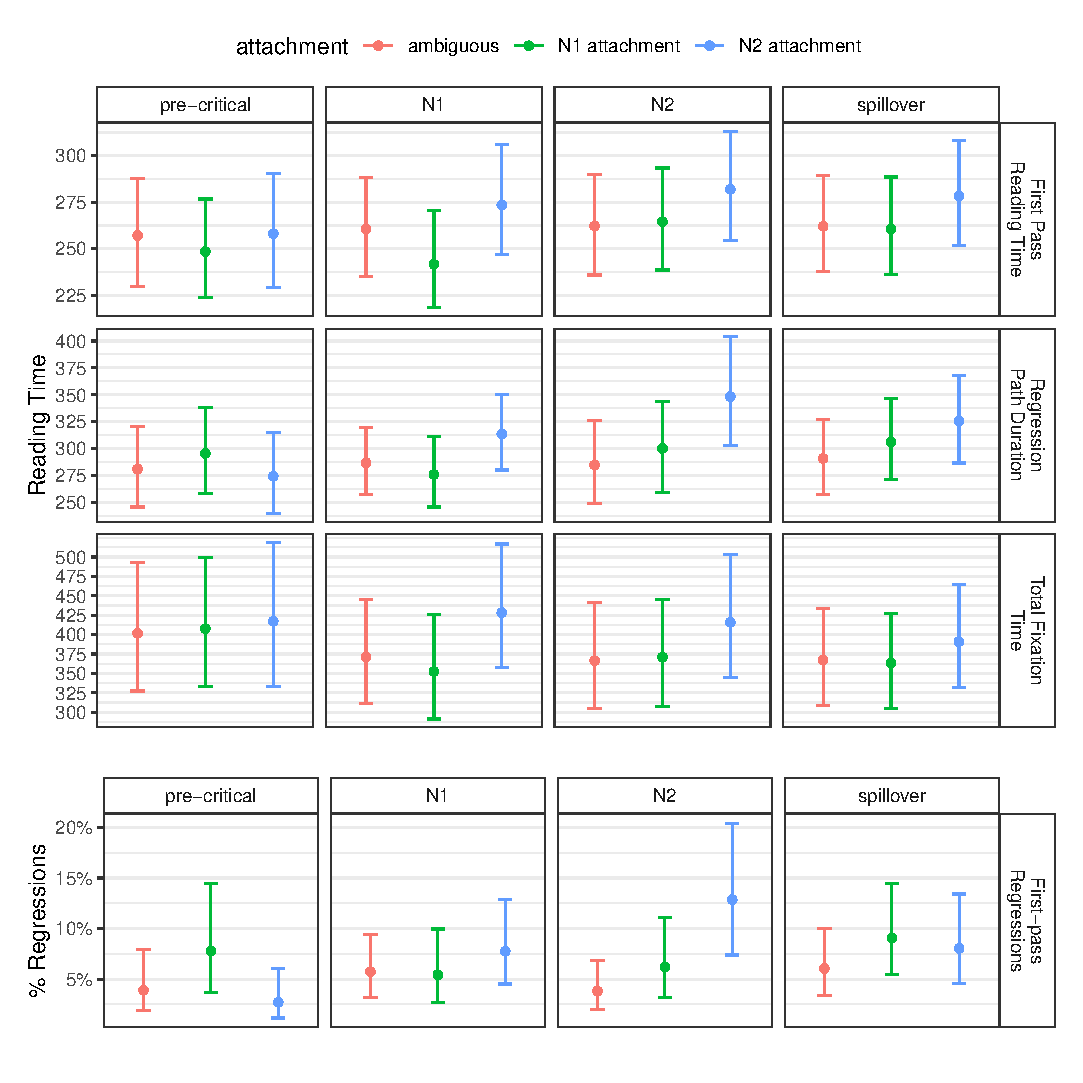
\includegraphics[width=\maxwidth]{figure/eyeEMM.eps} 
\caption{Estimated marginal means and 95\% credible intervals of first-pass regression probabilities and back-transformed log-reading time measures FPRT, RPD, and TFT for the critical regions by condition. All estimates and credible intervals were obtained using the \protect\texttt{emmeans} package \protect\citep{emmeans}.
%\protect{\citep{emmeans}}.
}
\label{fig:EyeRTsPlot}
\end{figure}

\begin{figure}
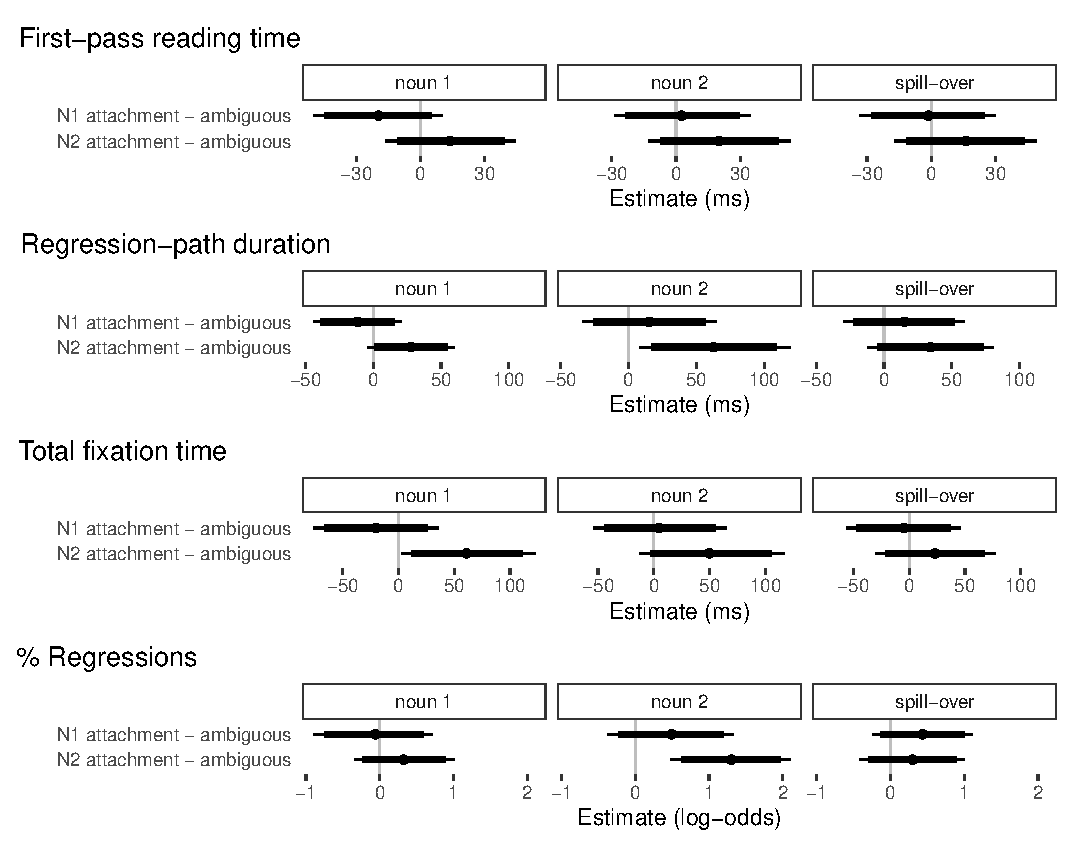
\includegraphics[width=\maxwidth]{figure/emStandardMeasuresModelCoefPlot.eps} 
\caption{Estimates and $95\%$ credible intervals (thin lines) as well as $90\%$ credible intervals (thick lines)  for the analyses of first-pass reading time, regression-path duration, total fixation time, and regression probability.}
\label{fig:emStandardMeasuresModelCoefPlot}
\end{figure}


\begin{figure}
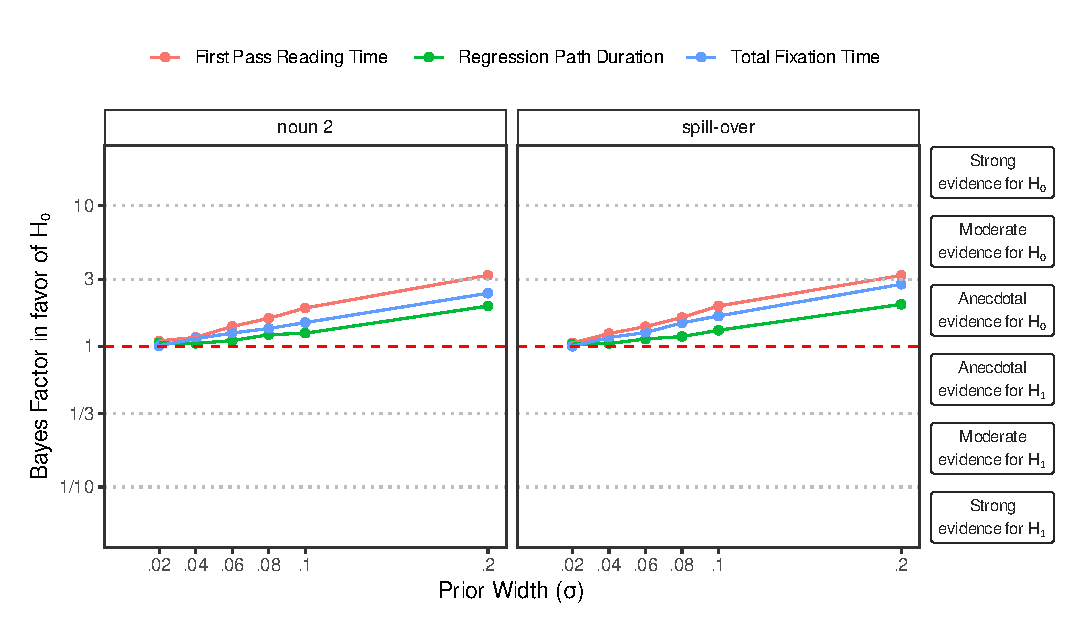
\includegraphics[width=\maxwidth]{./figure/exp1_BFs.eps} 
\caption{Bayes Factors in favor of the absence of a difference in reading times between the ambiguous attachment condition and the N1 attachment condition, at two positions in the sentence: noun 2 and the spill-over region. Classification of evidence strength following \citet{Jeffreys:1961} as cited in \protect\citet{LeeWagenmakers:2014}. }
\label{fig:EyeBFs1}
\end{figure}


The average comprehension questions accuracy was \(78.8\%\). \redx{Figure} \ref{fig:EyeRTsPlot} \redx{show} a summary of the {\hl estimated marginal means and 95\% credible intervals of the eye-tracking measures computed for the the critical regions using the \texttt{emmeans} package \citep{emmeans}:}
(i) \emph{First-pass reading time} (FPRT), which is the amount of time spent reading a word for the first time when that the first fixation on that word was \emph{progressive} (i.e., the reader has not yet read anything to the right of this word).
(ii) \emph{Regression-path duration} (RPD), which is the amount of time spent on the word starting with a progressive first fixation, until the gaze moves to the right of that word.
(iii) \emph{Total fixation time} (TFT), which is the total amount of time spent fixating the critical word, including re-reading.
(iv) The percentage of \emph{first-pass regressions}, which is the proportion of trials on which readers regress after reading the critical word).

Figure \ref{fig:emStandardMeasuresModelCoefPlot} shows the estimated differences between the unambiguous conditions and the ambiguous condition for each word position and eye-tracking measure. It also shows the upper and lower boundaries of the $95\%$ and $90\%$ credible interval for each position (noun 1, noun 2, spill-over region).\footnote{The posterior probability that the parameter is smaller than (or larger than) zero is larger than $97.5\%$ if the $95\%$ credible interval excludes zero and larger than $95\%$ if the $90\%$ credible interval excludes zero.}
%
The estimates indicate a slowdown in NP2 attachment conditions in first-pass reading times
(\textit{N2:} 
CrI [-13; 53], P($\beta$ > 0) =    .89;
% to-do: Fix all space-semicolon, and space-right parenthesis situations in the paper
\textit{spill-over:} 
CrI [-17; 49], P($\beta$ > 0) =    .84),
with stronger evidence for a slowdown in regression-path duration
(\textit{N2:} 
CrI [8; 119], P($\beta$ > 0) =    .99,
\textit{spill-over:} 
CrI [-12; 81], P($\beta$ > 0) =    .93).
In total fixation time, we found a slowdown in NP2 attachment conditions at N2
(CrI [-13; 117], P($\beta$ > 0) =    .94),
and an indication of an effect in the same direction at the spill-over region 
(CrI [-31; 77], P($\beta$ > 0) =    .81).
We further found an NP2 attachment-related slowdown in regression probability at N2
(CrI [-13.2; 117.3], P($\beta$ > 0) =    .94).

While most eye tracking measures at most regions reflected an NP2 attachment-related slowdown, only regression path duration and regression probability suggested a slowdown in the NP1 attachment conditions. Specifically, in RPD at N2
(CrI [-34; 65], P($\beta$ > 0) =    .74)
and at the spill-over region
(CrI [-30; 59], P($\beta$ > 0) =    .76),
as well as regression probability at N2
(CrI [-0.4; 1.3], P($\beta$ > 0) =    .88).

Figure \ref{fig:EyeBFs1} shows the Bayes Factors in favor of the hypothesis of no difference between NP1 attachment conditions and ambiguous conditions. While the Bayes Factor indicates a small amount of evidence for the hypothesis of \textit{no difference} between ambiguous and N1 attachment conditions for all but the most narrow prior ($\sigma=0.02$), it fails to provide unambiguous evidence in favor of that hypothesis.



\subsection{Discussion}

We found evidence for substantial processing difficulty in unambiguous NP2 attachment sentences relative to the ambiguous attachment condition, while the effect of unambiguous NP1 attachment was less clear. In the NP2 attachment condition, we found an indication of processing difficulty in most eye-tracking measures starting with regression path duration on N1, suggesting that reading in NP2 attachment sentences is initially slowed by the the fact that the RC cannot be attached to the first structurally available noun phrase, headed by N1. The subsequent slowdown relative to the ambiguous baseline may be due to the time the parser spends in carrying out RC attachment to the noun phrase headed by N2.

The results concerning the relative difficulty of the NP1 attachment sentences are less clear-cut: We found no appreciable slowdown in first-pass reading time or total fixation time at N2 in the NP1 attachment condition relative to the ambiguous condition. However, the regression path duration as well as the regression probability indicated somewhat higher processing difficulty in the NP1 attachment conditions compared to the ambiguous conditions. While the Bayes Factor analysis indicated weak evidence in favor of an absence of an ambiguity advantage, it failed to provide unambiguous evidence in favor of this hypothesis.


\section{Experiments {2A \& 2B}}

The second experiment was designed to address three issues which may complicate the interpretation of the first experiment: Firstly, although participants in Experiment 1 were asked only 5 comprehension questions about relative clause attachment, and only in unambiguous conditions, their presence may still have discouraged underspecification. Secondly, the analysis of multiple eye tracking measures at multiple regions increases the chances that one of them exhibits a theoretically interesting effect purely by chance, even in the absence of such an effect \cite[e.g.,][]{vonderMalsburgAngele:2017}. Lastly, a plausibility-based disambiguation of RC attachment may have caused between-participant or between-item variability in the time course of disambiguation, thus making its effect more difficult to detect.

In order to address these potential shortcomings, we conducted a self-paced reading experiment in which we asked only occasional superficial questions on one third of the trials, and used a different stimulus design. The experimental sentences in this experiment had a structure similar to sentence (\ref{ExpSPRExample}), in which the head noun of the relative clause (`\emph{football player'}/'\emph{fan'}) performs the function of the subject of the embedded verb (\emph{`hit'}). The grammatical object of all relative clauses was the reciprocal pronoun \emph{each other}. RC attachment was disambiguated by the grammatical number of the nouns in the complex noun phrase \emph{'fan(s) of the football player(s)'}. In (\ref{ExpSPRExample}), for instance, the relative clause \emph{'hit each other'} can attach to the NP headed by \emph{fans} because it is plural, but not to the NP headed by'\emph{football player'}, because it is singular and therefore cannot bind the reciprocal '\emph{each other'}.

\begin{exe}
\ex \label{ExpSPRExample}
\gll $[$Birbirini döven$]_{RC}$ futbolcu-nun hayran-lar-ı terk etti. \\
      {each other} hit  {footballer}.\textsc{sg}-\textsc{gen} {fan}-\textsc{pl}-\textsc{poss} leave did. \\
\textit{`The fan(s) of the football player(s) who hit each other left the stadium.'}
\end{exe}


We used the fact that relative clauses with a reciprocal as a grammatical object can only attach to plural noun phrases to create three attachment conditions: NP1 attachment, NP2 attachment and ambiguous attachment, as illustrated in (\ref{ExpSPRExperimental}). Because plurals were formed through the addition of the plural suffix \emph{-ler/-lar}, reading times for plurals and singulars may vary due to word length. In order to control for possible effects of length, we created three control conditions illustrated in (\ref{ExpSPRControl}) in which the complex noun phrase was modified by an adjective which could only attach to NP1. In the examples in (\ref{ExpSPRControl}) it is \emph{`Fenerbahçeli'} (meaning \emph{`of Fenerbahçe'}, a well-known Turkish football team). These additional conditions served as a baseline, and any differences between experimental conditions in (\ref{ExpSPRExperimental}) and control conditions in (\ref{ExpSPRControl}) may be considered effects of RC attachment.

As in Experiment 1, both underspecification accounts predict a speed-up in the ambiguous condition at the second noun, compared to the NP1 attachment condition. This prediction translates into an interaction between modifier type and the grammatical number of the second noun. That is, NP1 attachment sentences should exhibit a larger slowdown relative to their controls than the ambiguous condition relative to its control. In contrast, the SMCM as well as the late underspecification account, predict the absence of such an interaction. It predicts the absence of an ambiguity advantage, which means that there should not be any significant interaction between modifier type and the grammatical number of the second noun in the RC attachment conditions.

\begin{exe}
\ex \label{ExpSPRExperimental} 

\gll Dün akşam, \ldots \\
     Yesterday evening, {} \\
     
\begin{xlist} 

\item[a.]{}\textsc{ambiguous attachment (plural-plural)}{} 
\gll $[$birbirini döven$]_{RC}$ futbolcu-lar-ın hayran-lar-ı \\
{each other} hit {football player}-\textsc{pl}-\textsc{gen} {fan}-\textsc{pl}-\textsc{poss}  \\

\item[b.]{}\textsc{NP1 attachment (plural-singular)}{} 
\gll $[$birbirini döven$]_{RC}$ futbolcu-lar-ın hayran-ı \\
{each other} hit  {football player}-\textsc{pl}-\textsc{gen} {fan}.\textsc{sg}-\textsc{poss}  \\

\item[c.]{}\textsc{NP2 attachment (singular-plural)}{} 
\gll $[$birbirini döven$]_{RC}$ futbolcu-nun hayran-lar-ı\\
{each other} hit  {football player}.\textsc{sg}-\textsc{gen} {fan}-\textsc{pl}-\textsc{poss}  \\

\item[] \gll {\ldots} stadyumu hemen terk etti. \\
{}       stadium  immediately leave did. \\
\end{xlist}

\textit{`The fan(s) of the football player(s) who hit each other left the stadium immediately, yesterday evening.'}
\end{exe}

\begin{exe}
\ex \label{ExpSPRControl} 

\gll Dün akşam, \ldots \\
     Yesterday evening, {} \\
     
\begin{xlist} 

\item[a.]{}\textsc{ambiguous attachment control (plural-plural)}{} 
\gll $[$Fenerbahçe-li$]_{ADJ}$  futbolcu-lar-ın hayran-lar-ı \\
{Fenerbahce-\textsc{adj}} hit {football player}-\textsc{pl}-\textsc{gen} {fan}-\textsc{pl}-\textsc{poss}  \\

\item[b.]{}\textsc{NP1 attachment control (plural-singular)}{} 
\gll $[$Fenerbahçe-li$]_{ADJ}$  futbolcu-lar-ın hayran-ı \\
{Fenerbahce-\textsc{adj}} hit  {football player}-\textsc{pl}-\textsc{gen} {fan}.\textsc{sg}-\textsc{poss}  \\

\item[c.]{}\textsc{NP2 attachment control (singular-plural)}{} 
\gll $[$Fenerbahçe-li$]_{ADJ}$ futbolcu-nun hayran-lar-ı\\
{Fenerbahce-\textsc{adj}}  hit  {football player}.\textsc{sg}-\textsc{gen} {fan}-\textsc{pl}-\textsc{poss}  \\

\item[] \gll {\ldots} stadyumu hemen terk etti. \\
{}       stadium  immediately leave did. \\
\end{xlist}

\textit{`The fan(s) of the Fenerbahce football player(s) left the stadium immediately, yesterday evening.'}
\end{exe}



\subsection{Method}

\subsubsection{Materials}

Forty-two experimental sentence sets like (\ref{ExpSPRExperimental}) and (\ref{ExpSPRControl}) were constructed. All relative clauses comprised between two and three words and always started with a reciprocal pronoun. Sentences were divided into different lists according to a Latin-square design, such that every participant read exactly one sentence from each sentence set, and seven sentences from every condition. Experimental sentences were mixed with 65 filler sentences, so that every participant read 107 sentences during the course of the experiment. Each list was randomized prior to presentation.

\subsubsection{Participants}

The experiment was conducted in the lab (Experiment 2A) and online  (Experiment 2B) using the same stimuli. 
Participants in both experiments provided informed consent and the procedures in this study were compliant with the ethical principles outlined in the Helsinki Declaration on research involving human subjects.

\emph{\uline{Experiment 2A}.}
Thirty-six students of Anadolu University in Eskişehir, Turkey participated in the experiment. All participants were native speakers of Turkish, with an age range of 19-29 years. 

\emph{\uline{Experiment 2B}.}
A total of 148 students of four universities in Turkey participated in the experiment on-line in exchange for course credit (Boğaziçi University: 116, Ankara University: 13, Muğla Sıtkı Koçman University: 13, İstanbul Medipol Üniversitesi: 6). 
All participants were native speakers of Turkish, with an age range of 17-47 years (mean: 22 years). 



\subsubsection{Procedure}
The task was self-paced non-cumulative word-by-word reading. At the beginning of a trial, all words, masked by underscores, appeared. Participants pressed the space bar to reveal the next word. As the next word appeared, the current one was masked by underscores again. The time between key presses was recorded as the reading time for the word.
%
Each participant read five practice sentences before the start of the experiment.
Questions about the sentence were asked on one third of all trials (14 questions about experimental sentences, 21 questions about fillers). Participants answered questions with \texttt{`yes'} or \texttt{`no'} by pressing the corresponding button on the keyboard.

\emph{\uline{Experiment 2A}.}
Presentation and recording was done in a quiet room, using the Linger software package, version 2.94 by Doug Rohde. One experimental session took approximately 40 minutes to complete. Participants were paid 15 Turkish Lira for participation.

\emph{\uline{Experiment 2B}.}
The experiment was run online, using the web-based platform PCI Farm \citep{pcibex}. One experimental session took approximately 30 minutes to complete. 



\subsubsection{Statistical Analysis}

{\red
Because the experimental items were identical in Experiments 2A and 2B, we pooled the data from both experiments for the purposes of the statistical analysis in order to increase statistical power for detecting an ambiguity advantage effect.\footnote{We did not include a predictor for experiment modality (indicating \textit{`online'} or \textit{`in the lab'}) because potential interactions between the magnitude of a potential ambiguity advantage in Turkish and experiment modality are beyond the scope of this paper.} }  
%
We excluded the data of seven participants from Experiment 2B from further analysis because they failed to answer more than 25\% of the comprehension questions correctly. 
We also excluded all trials in which the reading time on one of the words between the pre-critical region and the spill-over region was shorter than $150\,ms$ or longer than $3000\,ms$, resulting in exclusion of further $2.2\%$ of the data ($170$ out of $7,644$ trials).

The data analysis followed the same logic as in Experiment 1:
All reading time measures were modeled using Bayesian generalized hierarchical linear models assuming log-normally distributed residuals 
%\citep[e.g.,][]{GelmanHill:2007, McElreath:2016, Kruschke:2015, VasishthEtAl:2019}.
We used a normal prior ($N(\mu=6, \sigma=1)$) for all model intercepts, and a symmetrical prior for all slope coefficients ($N(0, 0.2)$). All models were fitted using four chains with \(2,000\) warmup samples  \(5,000\) post-warmup samples each.


All models included fixed effects of 
(i) centered log-word length, 
(ii) the availability of NP1 and N2 for RC attachment, 
(iii) the presence of a relative clause (\emph{relative clause} vs.~\emph{control}), as well as 
(iv) the interactions between the presence of a relative clause and the availability of NP1 and NP2 for RC attachment.
Log word length was used as a covariate in order to account for any differences in critical word length between our experimental sentences. For word length at critical regions N1 and N2, the word length of the singular form was used. All contrasts were centered.
%
We included varying intercepts for participants and items, as well as maximal by-participant and near-maximal by-item slopes and correlations between random intercepts and slopes. 

The grammatical number of N1 and N2 which determined the potential availability of NP1 and NP2 for RC attachment when an RC was present was coded using centered contrasts. As a result, the relative difficulty of RC attachment in the three attachment conditions corresponded to the interactions between N1 and N2 number and the presence of a relative clause: (i) The interaction between the presence of an RC and N1 number corresponded to the difference between the effect of N1 number in the RC conditions ((\ref{ExpSPRExperimental}b) vs. (\ref{ExpSPRExperimental}a)) and its effect in the control conditions ((\ref{ExpSPRControl}b) vs. (\ref{ExpSPRControl}a)), that is, \emph{effect of NP1 attachment - effect of ambiguous attachment}.
(ii) Similarly, the interaction between the presence of an RC and N2 number corresponded to the difference between the effect of N2 number in the RC conditions ((\ref{ExpSPRExperimental}c) vs. (\ref{ExpSPRExperimental}a)) and its effect in the control conditions ((\ref{ExpSPRControl}c) vs. (\ref{ExpSPRControl}a)), that is \emph{effect of NP2 attachment - effect of ambiguous attachment}.
In sum, because the coefficients associated with the interaction contrasts represent the differences in the effect of NP1 and NP2 availability associated with the presence of a relative clause, they can be interpreted as the respective effects of unambiguous NP1 and NP2 attachment, relative to the ambiguous condition.

While all coefficients for reading time measures were on a log-scale, we used the model's posterior MCMC samples to construct 95\% credible intervals on the original scale (in \emph{milliseconds}).
% for (i) the main effect of relative clause attachment, as well as for (ii) the interactions between NP1 and NP2 unavailability and the presence of a relative clause, which correspond to the pairwise differences between each of the unambiguous conditions and the ambiguous condition. 
%Doing so allowed us to compare the size of the effects we found with previously attested instances of the ambiguity advantage.

As in Experiment 1, we used the Savage-Dickey method to calculate Bayes Factors quantifying the evidence against the presence of an ambiguity advantage for a range of priors. Because in this experiment, the critical parameter was the interaction between the presence of an RC and N1 number, we fitted all models with all priors in table \ref{tab:prior_widths}.

\subsection{Data Availability}
All data and R code used in the data analysis is available at \url{https://osf.io/r8dm7/}.


\subsection{Results}


\begin{figure}
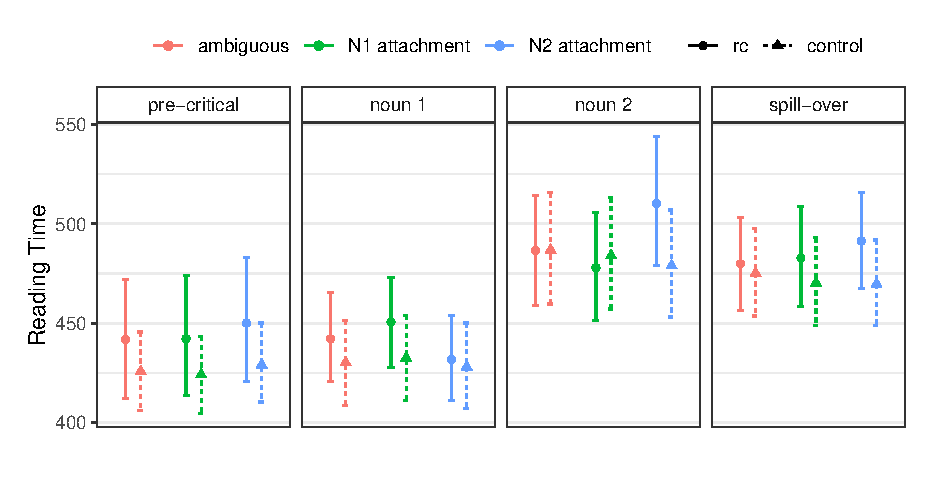
\includegraphics[width=\maxwidth]{./figure/sprEMMs.eps} 
\caption{Estimated marginal means and 95\% credible intervals of back-transformed log-reading time for the critical regions by condition. All estimates and credible intervals were obtained using the \texttt{emmeans} package 
\protect{\citep{emmeans}}. }
\label{fig:sprAverageRTs}
\end{figure}

\begin{figure}
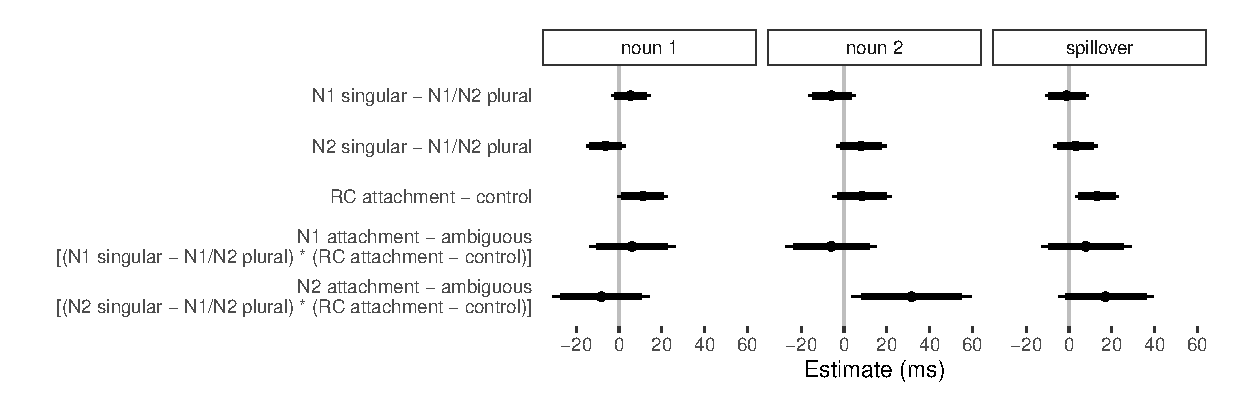
\includegraphics[width=\maxwidth]{figure/sprModelPlot.eps} 
\caption{Estimates and $95\%$ credible intervals (thin lines) as well as $90\%$ credible intervals (thick lines) for the effect (in milliseconds) of unambiguous RC attachment relative to ambiguous attachment on reading times at the critical regions.}
\label{fig:sprModelPlot}
\end{figure}

\begin{figure}
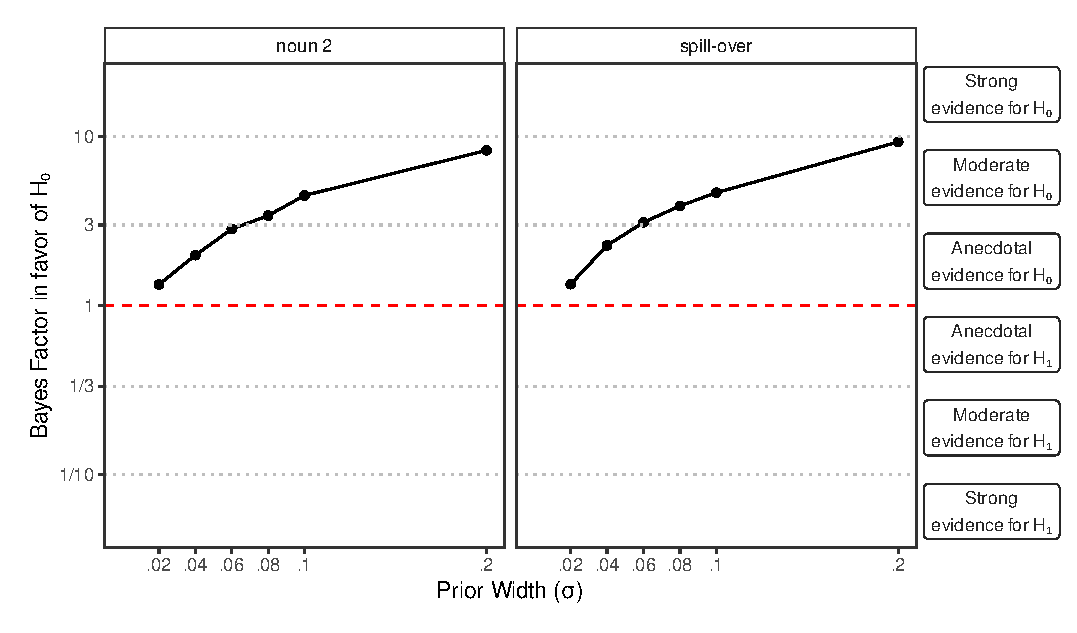
\includegraphics[width=\maxwidth]{./figure/exp2_BFs.eps} 
\caption{Bayes Factors in favor of the absence of a difference in reading times between the ambiguous attachment condition and the N1 attachment condition, at two positions in the sentence: noun 2 and the spill-over region. Classification of evidence strength following \citet{Jeffreys:1961} as cited in \citet{LeeWagenmakers:2014}.
}
\label{fig:EyeBFs2}
\end{figure}


Figure \ref{fig:sprAverageRTs} shows the average log-reading times transformed back to the original scale (milliseconds). Figure \ref{fig:sprModelPlot} shows the estimates and $95\%$ and $90\%$ credible intervals for the key contrasts at the critical regions in milliseconds.
The effects of RC attachment correspond to the interactions between the presence of a relative clause and the contrasts encoding the grammatical number of N1 and N2.\footnote{The posterior probability that the parameter is smaller than (or larger than) zero is larger than $97.5\%$ if the $95\%$ credible interval excludes zero and larger than $95\%$ if the $90\%$ credible interval excludes zero.}

As figure \ref{fig:sprModelPlot} shows, 
we found that N1 and N2 were read faster in their singular form than in in their plural forms 
(\emph{N1:} 
CrI [-4; 15], P($\beta$ > 0) =    .88,
\emph{N2:} 
CrI [-15; 3], P($\beta$ > 0) =    .09). 
%
Moreover, it shows an across-the-board slowdown in reading in RC attachment conditions compared to control conditions
(\emph{N1:}
CrI [-1; 23], P($\beta$ > 0) =    .97,
\emph{N2:}
CrI [-5; 22], P($\beta$ > 0) =    .89,
\emph{spill-over:}
CrI [3; 23], P($\beta$ > 0) =   .995).

We found no indication of differences in reading time between the \emph{NP1 attachment condition} and the ambiguous attachment condition.
%
However, we observed a slowdown in the \emph{NP2 attachment condition} relative to the ambiguous condition at N2
(CrI [4; 60], P($\beta$ > 0) =    .99)
and at the spill-over region
(CrI [-5; 40], P($\beta$ > 0) =    .93).

The posterior probability that the ambiguity advantage effect (the difference between the NP1 attachment and the ambiguous condition) was larger than the smallest ambiguity advantage attested in the literature ($3\%$) was
(\(P(log~\beta \geq 0.03 ) = 0.03 \), 
\(P(\beta \geq 22\,ms ) = 
    0.01
  \))
at N2, and
(\(P(log~\beta \geq 0.03 ) = 0.10 \), 
\(P(\beta \geq 22\,ms ) = 
    0.09
  \))
at the spill-over region.

Figure \ref{fig:EyeBFs2} shows Bayes Factors for the absence of a difference between ambiguous and N1 attachment conditions.
The analysis shows a moderate or near-moderate amount of evidence against models with 
$\sigma=0.2/0.1/0.08/0.06$: All $BF$s were $>3$ with the exception of the $BF$ for $\sigma=0.06$ at the N2 region, which was $BF_{01}=2.8$. Meanwhile, the evidence against models with $\sigma=0.04$ is relatively weak (\emph{N2:} $BF_{01} = 2$, \emph{spill-over:}  $BF_{01} = 2.3$) and the evidence against models with $\sigma=0.02$ was very weak
(\emph{N2:} $BF_{01} = 1.3$, \emph{spill-over:}  $BF_{01} = 1.3$).



\subsection{Discussion}

We found an across-the-board slowdown in relative clause attachment conditions compared to the control conditions, which likely reflects the increased processing difficulty associated with the processing and attachment of relative clauses, compared to adjectives. We further found evidence for a slowdown at N2 and the spill-over region in NP2 attachment sentences. As in experiment 1, this finding likely reflects late RC attachment in the NP2 attachment condition. 


Importantly, our data did not indicate the presence of an effect of a magnitude which was comparable to previously attested instances of an ambiguity advantage. We had hypothesized that such an effect would occur either at N2 or at the spillover position. The posterior probability of an ambiguity advantage of the smallest expected magnitude at N2 was very low
($0.005$), and relatively low ($0.09$) at the spill-over region.
Moreover, the Bayes Factor analysis provided a moderate level of evidence against nearly all models allocating a substantial amount of probability mass to an effect size between $3\%$ and $19\%$. 
%
The only models for which the Bayes Factors in favor of the absence of an effect were \emph{anecdotal} (but positive) $\sigma=0.04$ and $\sigma=0.02$, which allocated a relatively large amount of probability mass to effect sizes below $3\%$ ($.77$ and $.93$, respectively), and a relatively low amount of probability mass to effect sizes above $3\%$  ($.23$ and $.07$, respectively).
These findings suggest that either the structure studied in this experiment does not elicit an ambiguity advantage or if it does, its effect size is most likely substantially smaller than previously attested instances.



\section{General Discussion}

We conducted two reading experiments to test a prediction made by the strategic underspecification account: underspecification of attachment in structures with prenominal relative clauses.
If readers strategically underspecify ambiguous sentences, they should do so even when RCs are prenominal, as they are in Turkish. Therefore, under the assumption of strategic underspecification, we expected to observe an ambiguity advantage in prenominal relative clauses. Under a race-based account such as the SMCM, however, no ambiguity advantage was expected.

In Experiment 1 (N=$36$), we tested this prediction in an eye tracking experiment in which a relative clause attachment ambiguity was disambiguated by means of plausibility. We did not find clear-cut evidence for or against an ambiguity advantage in this experiment. While the first-pass reading time and the total fixation time at the critical region did not indicate shorter processing times in ambiguous sentences compared to the preferred NP1 attachment conditions, the regression path duration as well as the number of first-pass regressions pointed to a potential, albeit small speedup. 
A Bayes Factor analysis failed to provide conclusive evidence for or against a difference in reading times between ambiguous and N1 attachment conditions, although it did provide tentative evidence against a \textit{substantial} speedup. 
This finding is consistent with the absence of an ambiguity advantage, as well as with the presence of a relatively small ambiguity advantage.

In Experiment 2, we tested the same prediction as in Experiment 1 with a different experiment design and a substantially increased number of participants (N=$184$). We found no evidence for the presence of an ambiguity advantage. Moreover, additional analyses based on (i) the posterior of the estimate of the difference between the ambiguous and N1 attachment conditions, and (ii) on a Bayes Factor analysis provide evidence against the presence of an ambiguity advantage of the magnitude that has previously been reported for English ($22\,ms-120\,ms$).

These findings present a challenge for both interpretations of the underspecification account by Swets et al.~(2008). When task demands do not encourage disambiguation, \emph{early underspecification} predicts an ambiguity advantage at NP2. This is because RC attachment is initially underspecified and later resolved in the NP2 attachment condition, but remains underspecified in the NP1 attachment condition. This should lead to a speedup in the ambiguous condition relative to the unambiguous NP1 condition. \emph{Late underspecification} predicts that the parser delays the process of attaching the RC until such a point where it knows with certainty whether the structure is ambiguous. Based on that information, it decides to underspecify RC attachment in ambiguous conditions, and to attach the RC in unambiguous attachment conditions. This is expected to happen either at the second noun or at the spill-over region. 
Since our findings in Experiment 2 reflect either the absence of an ambiguity advantage or a significantly reduced effect size, they pose a challenge for the underspecification account. If they reflect the absence of an effect, the findings are at odds as they indicate the absence of underspecification in structures with prenominal RCs.
The presence of an ambiguity advantage of a reduced magnitude, on the other hand, has two possible interpretations: Either underspecification occurs, but significantly less often than in English, thus leading to a decreased average effect, or the relative speed-up due to the underspecification of RC attachment is significantly smaller in Turkish than in English.
In either case, is not currently clear what factors are responsible for the the difference between postnominal and prenominal structures.

Importantly, race-based models such as the SMCM \citep{LogacevVasishth:2016} do not predict an ambiguity advantage in ambiguous structures with prenominal RCs because they assume that RC attachment begins at the earliest opportunity, which means that an attempt to attach the RC to NP2 must begin with a significant delay relative to the attempt to attach it to NP1. As a result, the chance that attachment to NP2 will be completed first is negligible, and no ambiguity advantage is expected. Thus, our findings are compatible with the SMCM, but pose a number of challenges for the underspecification account.


\section{Conclusion}

We proposed two different interpretations of the Swets et al. (2008) strategic underspecification account and discussed how the ambiguity advantage follows from their specific sets of assumptions.  
We argued that in contrast to race-based theories, both implementations of the strategic underspecification account predict an ambiguity advantage not only in languages with postnominal RCs, like English, but also in languages with prenominal RCs, such as Turkish.
We further presented the results of two reading time experiments which failed to show an ambiguity advantage comparable in magnitude with previously attested instances of the ambiguity advantage. 
We argue that our findings present a major challenge for the strategic underspecification account, but are compatible with race-based models such as the SMCM.



\bibliographystyle{apacite} 
\bibliography{library.bib}



\end{document}
